\chapter{Text Mining}\label{Text Mining}

Nu men een algemeen begrip heeft van wat machine learning juist is en welke algemene technieken het omvat, kan men overgaan naar text mining en zijn geschikte technieken. In dit hoofdstuk gaat men bespreken welke technieken men kan gebruken voor text mining en wat deze juist inhouden. Als laatste gaat men de theorie toepassen op een voorbeeld en gaat men de resultaten van dit experiment bespreken. 


Text mining of text data mining is een techniek waarbij men aan tekstanalyse doet om zo trends en patronen te kunnn vaststelllen. Neem opnieuw als voorbeeld onze artikels. Met text mining wil men de artikels zodanig analyseren zodanig dat men kan uitmaken welk artikel positief en welk negatief is.
Een probleem dat zich onmiddelijk bij text mining voordoet is het ontbreken van een  \'e\'en-op-\'en relatie van woorden en een concept. Woorden verwijzen zelfden eenduidig naar één concept. Zo het voorkomen van het woord "bank" in een tekst zowel verwijzen naar de finaciele instelling als naar een doodgewone zitbank in het park. Dergelijke dubbele betekenis van woorden maakt het moeilijk om de woorden, met als gevolg ook de tekst, te mappen op een bepaald concept.

Verder heeft men ook woorden in een tekst die weinig bijdragen tot de bepaling van het concept van de tekst bijvoorbeeld: ik,en,want...
Deze woorden kan men uit de tekst filteren door een database aan te leggen met woorden die moeten men moet negeren. Deze techniek en nog soortgelijke alternatieven vereisen dat er al een voorverwerking plaatsvindt voordat men de dataset echt gaat analyseren op patronenen trends. Algemeen kan men zeggen als men de resultaten van de text mining wil optimaliseren, men aan \textbf{\textit{document pre-processing}} moet doen.

\section{Document Pre-processing }\label{Document Pre-processing}

Document pre-processing is een optionele, maar zeker nuttig stap in het text mining proces. Document pre-processing bestaat eruit om je dataset al eens te verwerken, zodanig je extra informatie hebt, die je kan gebruiken bij de eigelijke analyse van de dataset. Zo kan je bijvoorbeeld alle stopwoorden verwijderen uit de dataset. Wanneer men dan op deze gewijzigde dataset een analyze uitvoert, geeft men indirect de informatie mee dat stopwoorden er niet toe doen. Uiteraard is het verwijderen van stopwoorden \'e\'en van de technieken.  Er bestaan nog andere technieken die nuttig zijn als voorverwerking van een dataset. Zo kan men tekst en stucturen afleiden. Bijvoorbeeld het omzetten van Microsoft Word of Latex documenten naar XML maakt het parsen en analyseren van de documenten voor het algoritme veel gemakkelijker.Verder kan men ook \textbf{\textit{stemming}} toepassen. Stemming is een techniek waarbij men tracht om de stam van het woord te achterhalen. Bijvoorbeeld uit het woord \textit{katachtig} kan men het woord \textit{kat} afleiden. De techniek kan gebaseerd zijn op een woordenboek bijvoorbeeld \textit{Mmorph} is zo'n stemming woordenboek ontwikkeld door de Universiteit van Gen\`eve. Verder kan men de stemming ook baseren op een set van regels, bepaald door taalkundige. Het onderstaande voorbeeld illustreert een set van stemming regels voor het Frans:

%Voorbeeld van stemming regels   
\newline
\begin{center}
  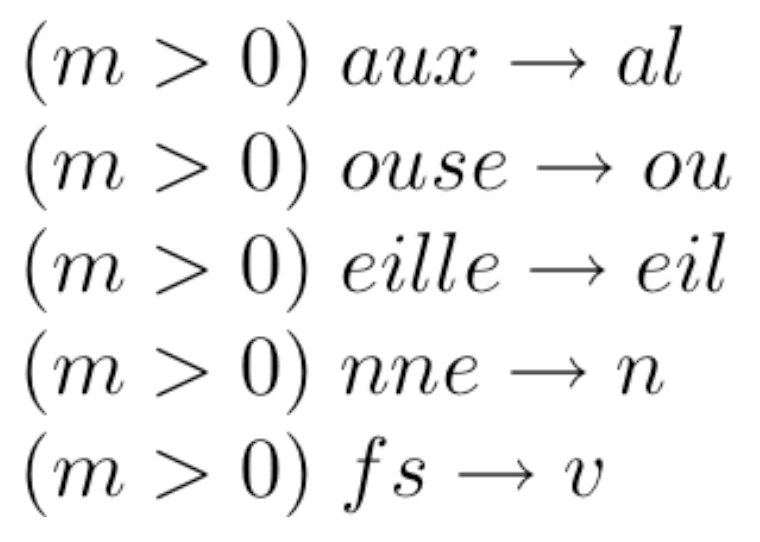
\includegraphics[width=5cm]{stemming_regels_frans}
  \captionof{figure}{Voorbeeld van stemming regels in het Frans}
\end{center}
%%
Tenslotte is \textbf{\textit{named entity recognition}} (NER) ook een techniek die men kan gebruiken bij document pre-processing. Hierbij gaat men entiteiten proberen detecteren in de tekst en deze labelen. Neem bijvoorbeeld de zin \textit{Yannick heeft zich ingeschreven de richting Computerwetenschappen aan de Vrije Universiteit Brussel in 2012}. Men kan met NER de entiteiten eruit halen, labelen en volgend resultaat verkrijgen: \textit{$\text{[Yannick]}_{persoon}$ heeft zich ingeschreven de richting Computerwetenschappen aan de $\text{[Vrije Universiteit Brussel]}_{organisatie}$ in $\text{[2012]}_{tijdsaanduiding}$}
\newline
Algemeen ziet men dat al deze technieken samen worden gecombineerd, wat alleen maar de uiteindelijke resultaten ten goede komt. Hoe deze gecombineerd kunnen wordt in het onderstaande voorbeeld ge\"illustreerd. 
\newline
\begin{center}
  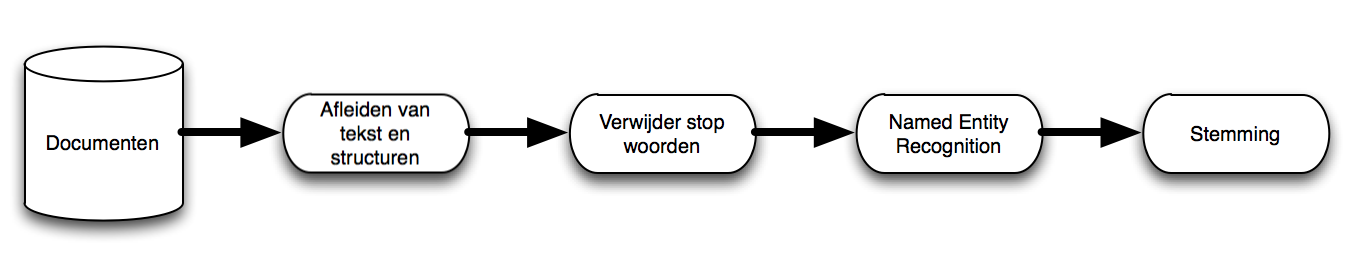
\includegraphics[width=10cm]{document_preprocessing}
  \captionof{figure}{Combinatie van technieken bij document pre-processing}
\end{center}

\section{Methoden}\label{Methoden}

\subsection{Vector Space Methode}\label{Vector Space Methode}


\subsubsection{Term weigthing}\label{Term weighting}

\subsubsection{Latent Semantic Models}\label{Latent Semantic Models}


\subsection{Probablistic methode}\label{Probablistic methode}

\section{LSA Experiment}\label{LSA Experiment}
